\section{Agent-based model Results}
\label{sec-cal}
\subsection{Calibration process}
We use optuna to perform the calibration. Each time, we sample parameters from the Tree-structured Parzen Estimator (TPE) sampler and run the simulation once. After that, we calculate the minimization objective value as the mean absolute error of the cumulative confirmed number between the simulation results and the real-world data and feed the  objective value to sampler. Because of the limitation of hardware and time, we times all the cases/deaths/vaccines with 0.01. We use the negative of mask policy indicator and the negative of residential mobility as the numerical mask policies and mobility value. We model the first outbreak (from March 2020 to Sept 2020) and the second outbreak (from July 2021 to Oct 25th) separately because they are caused by different variants.

For the first outbreak, we calibrate the following parameters:

\begin{itemize}
	\item $\beta_0$: the probability of a successful virus transmission per contact, calibration range is $[0.06,0.10]$.
	\item $\text{ma}_{\min}$: we calculate $a_1$ and $b_1$ such that $\max\{a_1x_{\text{ma}}+b_1)\}=1.0$ and $\min\{a_1x_{\text{ma}}+b_1)\}=\text{ma}_{\min}$. The calibration range is $[0.03, 0.25]$.
	\item $\text{mo}_{\min}$: we calculate $a_2$ and $b_2$ such that $\max\{a_2x_{\text{mo}}+b_2)\}=1.0$ and $\min\{a_2x_{\text{mo}}+b_2)\}=\text{mo}_{\min}$. The calibration range is $[0.1, 0.6]$.
	\item $\text{symp\_prob}$: the test probability of a symptomatic agent, calibration range is $[0.9,1.0]$.
	\item $\text{trace\_probs}$: the successful probability of a contact tracing, calibration range is $[0.75,0.99]$.
	\item $\text{start\_shift}$: the number of days between the first ten people get infected and the first confirmed case, calibration range is $[-8,8]$.
\end{itemize}

Besides these parameters, we set the following parameters as constants:
\begin{itemize}
	\item $\text{pop\_infected}=10$: the number of infected people at the start of the simulation
	\item $\text{asymp\_prob}=0$: the test probability of a asymptomatic agent
	\item $\text{quar\_period}=7$: the maximum quarantine time in days, we collect the value from the official \href{https://www.covid.gov.sg/exposed/hrw}{MOH website}
	\item $\text{test\_delay}=1$: the number of days for test results to be known
\end{itemize}

After calibrating the first outbreak, we setup the second outbreak with the same constants and the calibration results $\text{ma}_{\min}$, $\text{mo}_{\min}$, $\text{symp\_prob}$, $\text{trace\_probs}$ of the first outbreak. For the second outbreak, we only calibrate the $\beta_0$ value in range $[0.61,0.3]$ and the $\text{start\_shift}$ in range $[-21,21]$ while take the vaccinations into consideration. Instead of introducing infected populations at the start of the simulation, we introduce 10 people infected by delta variant on the day when the first case gets confirmed (24th August) shifted by  $\text{start\_shift}$.

Regards the vaccination, we assume that people only receive Pfizer COVID-19 vaccines and the order in which people get vaccinated is the descending order of people's age. We also assume that people who have received the first dose 21 days before have priority in receiving the second dose. We calibrate the first outbreak with 5000 samples and the second outbreak with 2000 samples.

After calibrating the second outbreak, we assume the daily vaccine doses, mask policies and mobility as the mean of the last 30 days and predict the epidemiology data of the next 30 days, which lies in the yellow area of Figure \ref{cal2}.
\subsection{Calibration results}
\begin{figure}[htbp]
	\centering
	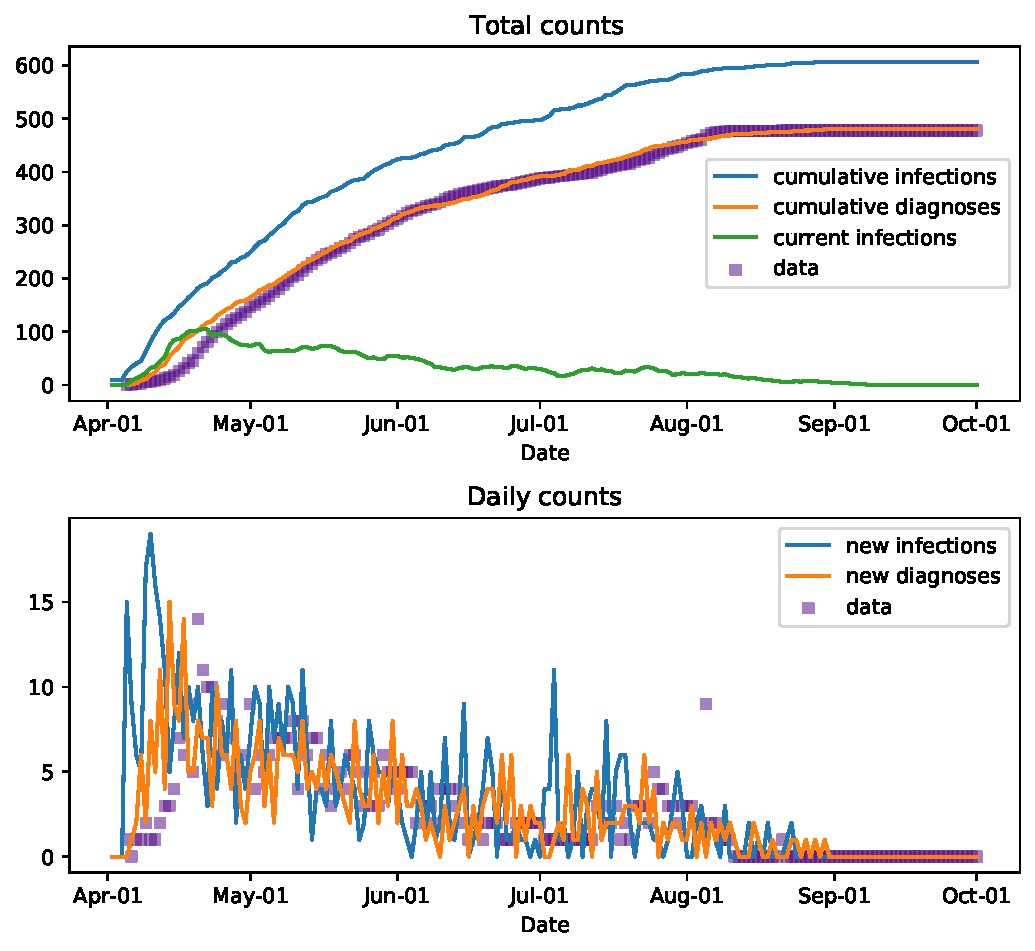
\includegraphics[width=0.95\linewidth]{result/sg_calib1_result.pdf}
	\caption{First outbreak, calibration results}
	\label{cal1}
\end{figure}
\begin{figure}
	\centering
	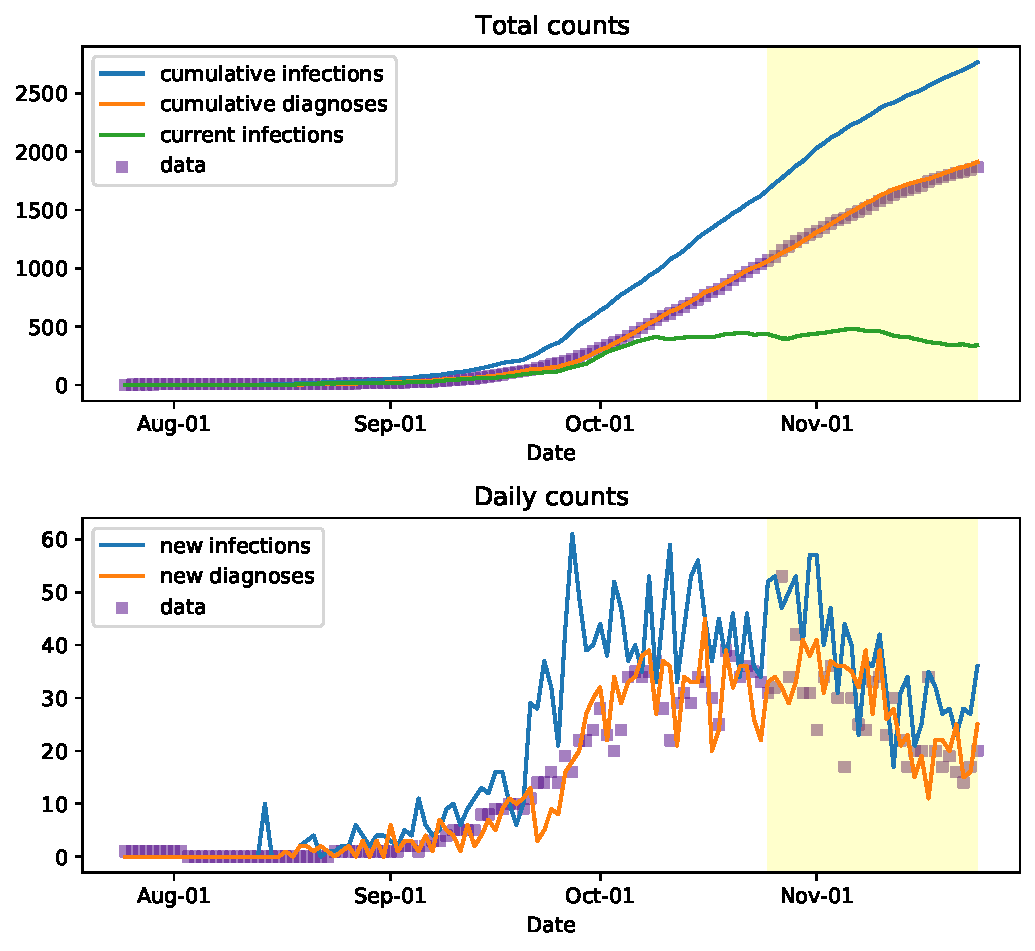
\includegraphics[width=0.95\linewidth]{result/sg_calib2_predict.pdf}
	\caption{Second outbreak, calibration results}
	\label{cal2}
\end{figure}
For the first outbreak, the calibrated parameters are $\beta_0=0.061$, $\text{ma}_{\min}=0.13$, $\text{mo}_{\min}=0.43$, $\text{symp\_prob}=0.9$, $\text{trace\_prob}=0.79$, $\text{start\_shift}=3$. Figure \ref{cal1} shows the calibration results of the first outbreak. The calibration results fit the data pretty well except the first month, which may results from the relatively low testing probability at the beginning.

For the second outbreak, the calibrated parameters are $\beta_0=0.134$, $\text{start\_shift}=10$. Figure \ref{cal2} shows the calibration results of the first outbreak and the prediction of the next 30 days (in yellow area). The calibration results not only fit the data well but also give a pretty good prediction. Cause the $\beta_0$ value has already been multiplied by 2.2 within covasim, the real $\beta_0$ value is $2.2\times 0.134\approx0.295$, which is about four times larger than the $\beta_0$ value of the first outbreak.
\subsection{Effect of vaccination}
\begin{figure}
	\centering
	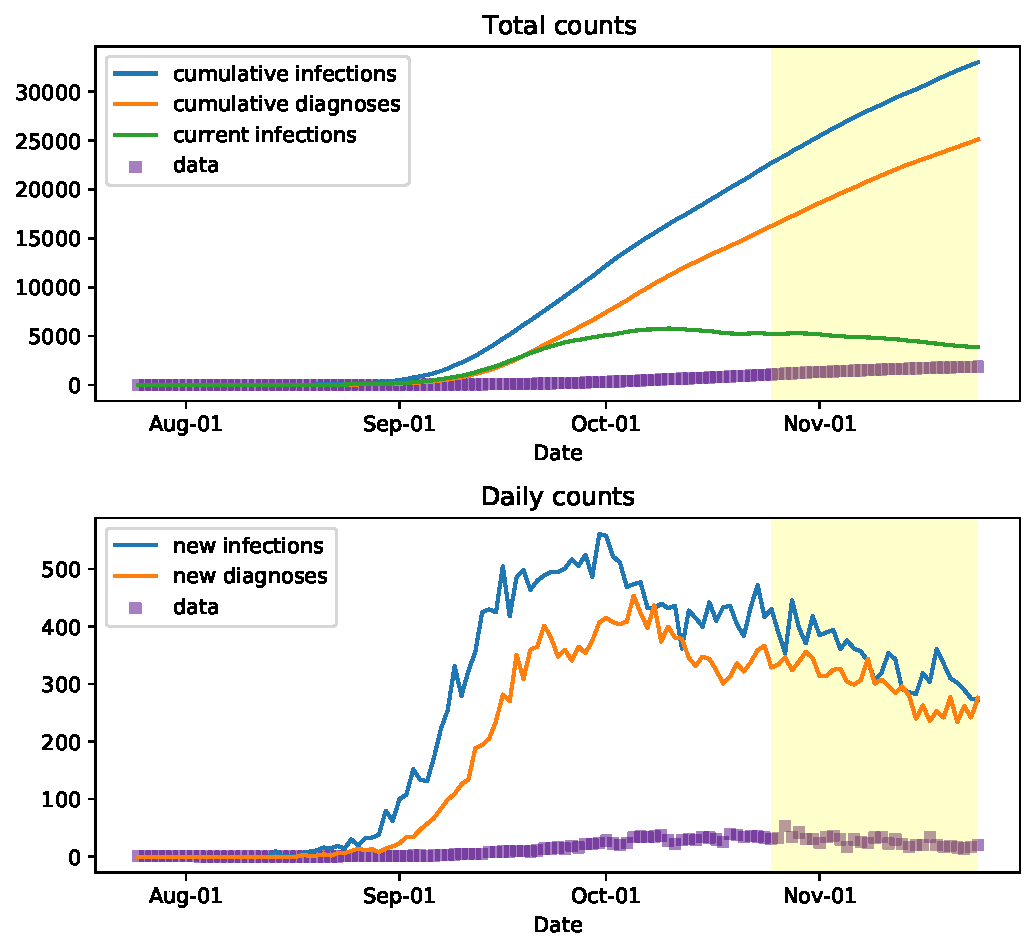
\includegraphics[width=0.95\linewidth]{result/sg2_zero_predict.pdf}
	\caption{Second outbreak, without vaccination}
	\label{without}
\end{figure}
To evaluate the effect of the vaccination, we run the simulation of the second outbreak with same parameters but without vaccination. Figure \ref{without} indicates that more than a half of the total population will get infected under such mask policies and mobility, which reveals the importance of the vaccination.
\subsection{Effect of mask policies and mobility}
\begin{figure}
	\centering
	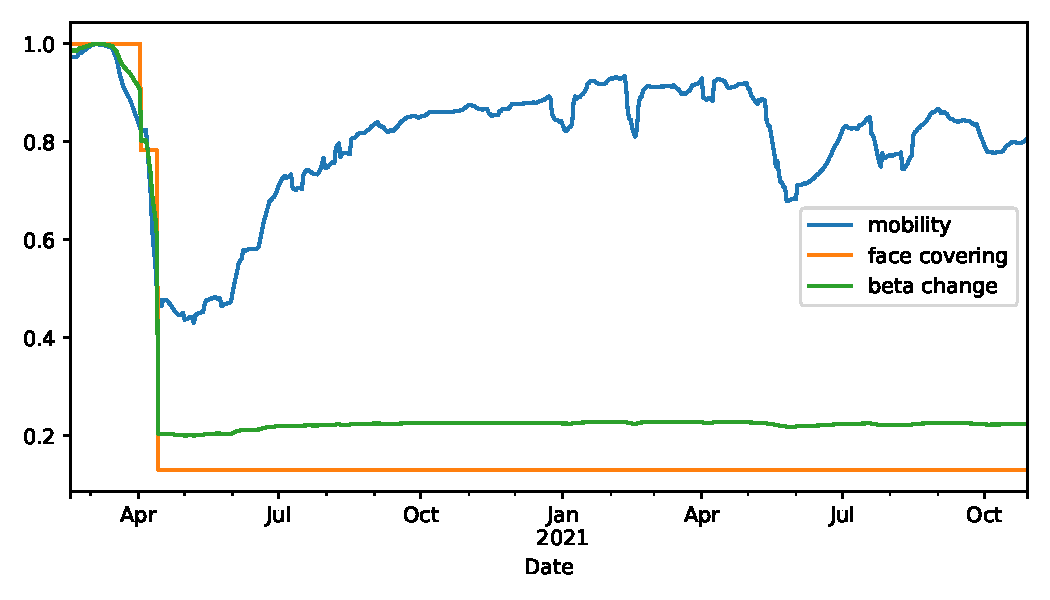
\includegraphics[width=0.95\linewidth]{result/sg_calib1_change.pdf}
	\caption{The impact of mask policies and mobility}
	\label{change}
\end{figure}
Figure \ref{change} shows the impact of mask policies and mobility on the $\beta$ value. When the mask policies are not strict, the change of mobility explains the main part of the change of $\beta$. However, when the mask policies becomes strict after mid-April, the change of mobility only causes small fluctuations on $\beta$.
